% LaTeX Template for Project Report, Version 2.0
% (Abstracted from a Major Project Report at CSED, NIT Calicut but can be
% modified easily to use for other reports also.)
%
% Released under Creative Commons Attribution license (CC-BY)
% Info: http://creativecommons.org/licenses/by/3.0/
%
% Created by: Kartik Singhal
% BTech CSE Batch of 2009-13
% NIT Calicut
% Contact Info: kartiksinghal@gmail.com
%
% It is advisable to learn the basics of LaTeX before using this template.
% A good resource to start with is http://en.wikibooks.org/wiki/LaTeX/
%
% All template fields are marked with a pair of angular brackets e.g. <title here>
% except for the ones defining citation names in ref.tex.
%
% Empty space after chapter/section/subsection titles can be used to insert text.
%
% Just compile this file using pdflatex after making all required changes.

\documentclass[12pt,a4paper]{report}
\usepackage{fullpage}
\usepackage{hyperref}
\usepackage{color}
\usepackage[pdftex]{graphicx}
\usepackage{todonotes}
\usepackage{ourmacros}
\usepackage{listings}
\usepackage{amsfonts}
\usepackage{amsmath}
\usepackage{url}
\usepackage{epstopdf} %What's this???
%\usepackage{hyperref}
%\usepackage[bookmarks, colorlinks=false, pdfborder={0 0 0}, pdftitle={<pdf title here>}, pdfauthor={<author's name here>}, pdfsubject={<subject here>}, pdfkeywords={<keywords here>}]{hyperref} %for creating links in the pdf version and other additional pdf attributes, no effect on the printed document
%\usepackage[final]{pdfpages} %for embedding another pdf, remove if not required

% Load the package
\usepackage[xindy]{glossaries}

% Generate the glossary
\makeglossaries

\begin{document}
%include other pages
% % % % % % % % % % % % % % % % % % % % % % % % % % % % % % % % % % %
% Term definitions
%
%     \newglossaryentry{<label>}{<settings>}
%
% Example
%
\newglossaryentry{computer}
{
	name=computer,
	description={is a programmable machine that receives input,
		stores and manipulates data, and provides
		output in a useful format}
}
%
%
% Defining acronyms
%
%    \newacronym{<label>}{<abbrv>}{<full>}
%
% Example
%
\newacronym{lvm}{LVM}{Logical Volume Manager}
%
% Use
%
%    \gls{computer}
%    \gls{lvm}
%
% % % % % % % % % % % % % % % % % % % % % % % % % % % % % % % % % % %



%\renewcommand\bibname{References} %Renames "Bibliography" to "References" on ref page
\listoftodos

%include other pages
\begin{titlepage}
	\begin{center}
		\textup{\small {\bf MI7 Project}}\\[0.2in]	
		% Title
		\Large \textbf {Learning Probabilistic Automata}\\[0.5in]
		
		\begin{figure}[!h]
			\centering
			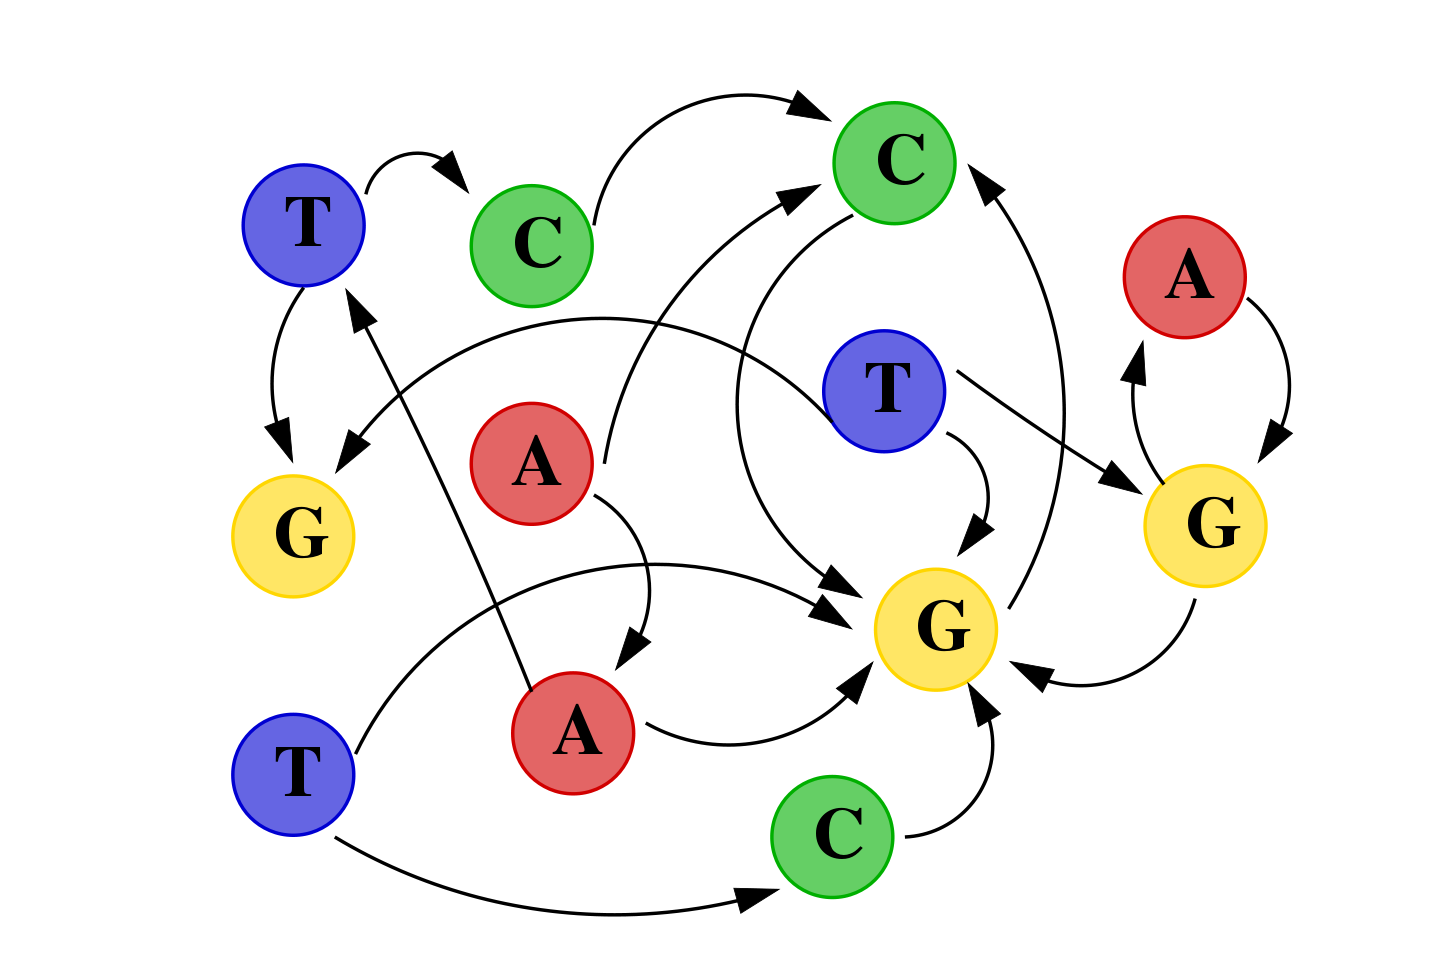
\includegraphics[width=1\linewidth]{pictures/Frontpage}
			\label{fig:Frontpage}
		\end{figure}
	\end{center}
\end{titlepage}


%\newpage
\thispagestyle{empty}

\begin{center}

\huge{Department of Computer Science and Engineering}\\[0.5cm]
\normalsize
\textsc{National Institute of Technology Calicut}\\[2.0cm]

\emph{\LARGE Certificate}\\[2.5cm]
\end{center}
\normalsize This is to certify that this is a bonafide record of the project presented by the students whose names are given below during <Monsoon/Winter and Year here> in partial fulfilment of the requirements of the degree of Bachelor of Technology in Computer Science and Engineering.\\[1.0cm]

\begin{table}[h]
\centering
\begin{tabular}{lr}
Roll No & Names of Students \\ \\ \hline
\\
<Roll no here> & <Name here> \\ 
<Roll no here> & <Name here> \\
<Roll no here> & <Name here> \\
\end{tabular}
\end{table}

\vfill


% Bottom of the page
\begin{flushright}
<Guide name here>\\
(Project Guide)\\[1.5cm]
<Coordinator name here>\\
(Course Coordinator)\\
\end{flushright}

\begin{flushleft}
Date:
\end{flushleft}

\vspace{2in}
\begin{abstract}

<Abstract here>

\end{abstract} 



\pagenumbering{roman} %numbering before main content starts
\tableofcontents
\listoffigures

\newpage
\pagenumbering{arabic} %reset numbering to normal for the main content




\begin{titlepage}
	\begin{center}
		\textup{\small {\bf MI7 Project}}\\[0.2in]	
		% Title
		\Large \textbf {Learning Probabilistic Automata}\\[0.5in]
		
		\begin{figure}[!h]
			\centering
			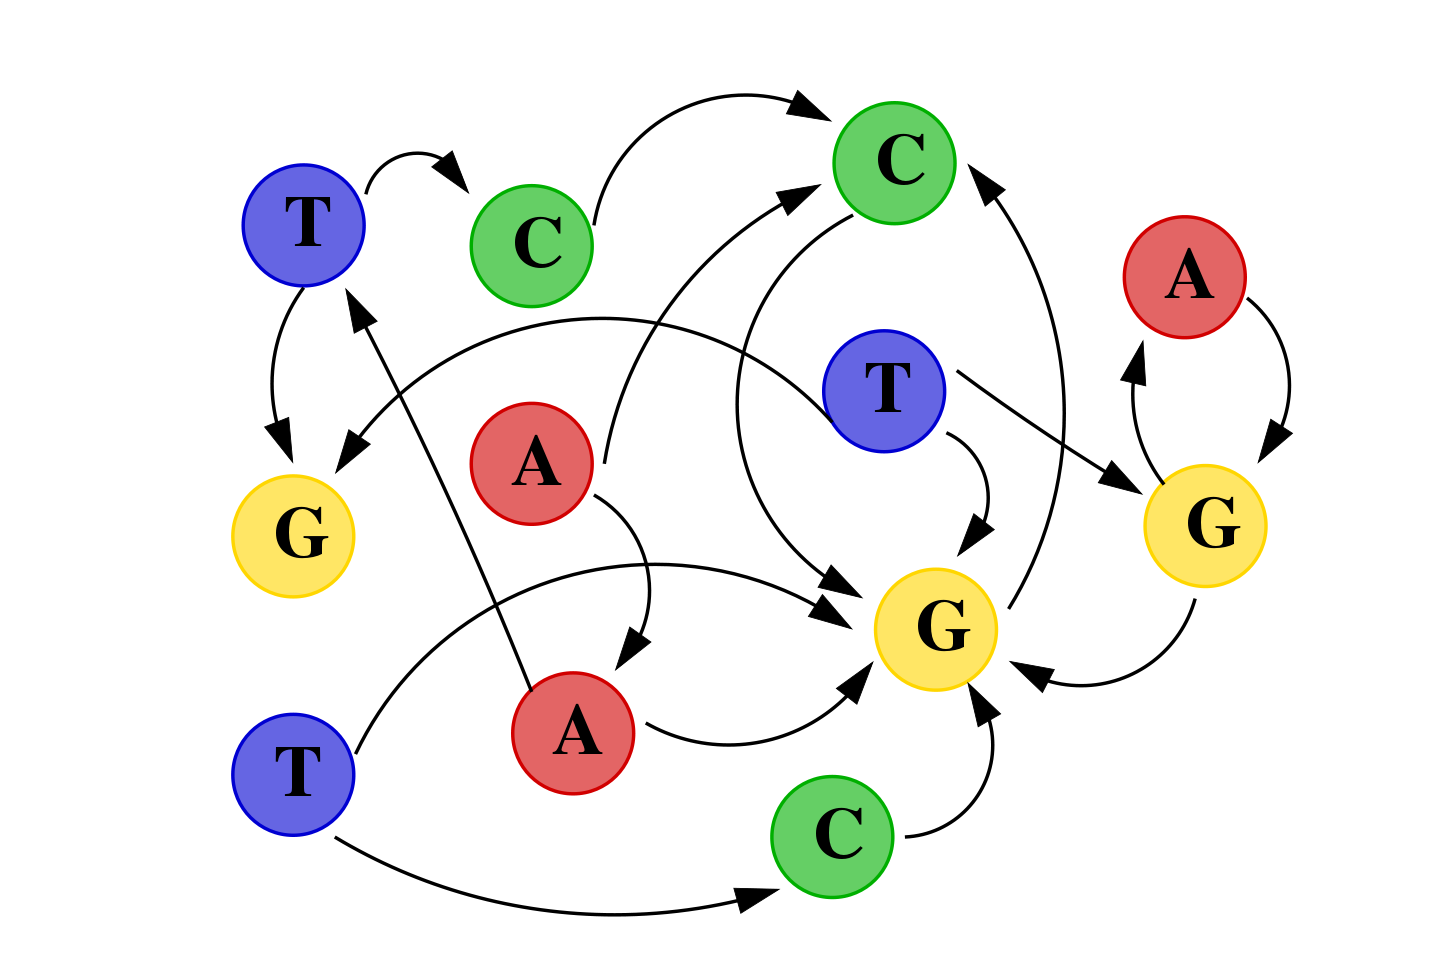
\includegraphics[width=1\linewidth]{pictures/Frontpage}
			\label{fig:Frontpage}
		\end{figure}
	\end{center}
\end{titlepage}

\newpage
\thispagestyle{empty}

\begin{center}

\huge{Department of Computer Science and Engineering}\\[0.5cm]
\normalsize
\textsc{National Institute of Technology Calicut}\\[2.0cm]

\emph{\LARGE Certificate}\\[2.5cm]
\end{center}
\normalsize This is to certify that this is a bonafide record of the project presented by the students whose names are given below during <Monsoon/Winter and Year here> in partial fulfilment of the requirements of the degree of Bachelor of Technology in Computer Science and Engineering.\\[1.0cm]

\begin{table}[h]
\centering
\begin{tabular}{lr}
Roll No & Names of Students \\ \\ \hline
\\
<Roll no here> & <Name here> \\ 
<Roll no here> & <Name here> \\
<Roll no here> & <Name here> \\
\end{tabular}
\end{table}

\vfill


% Bottom of the page
\begin{flushright}
<Guide name here>\\
(Project Guide)\\[1.5cm]
<Coordinator name here>\\
(Course Coordinator)\\
\end{flushright}

\begin{flushleft}
Date:
\end{flushleft}

\vspace{2in}
\begin{abstract}

<Abstract here>

\end{abstract} 


\pagenumbering{roman} %numbering before main content starts
\tableofcontents
\listoffigures

\newpage
\pagenumbering{arabic} %reset numbering to normal for the main content

\chapter{Introduction}

 %literature survey included in this

\chapter{Analysis}

\subsubsection{Avoiding zero values}

When training a model it is not certain that all possible sequences of symbols are read. Because of this uncertainty there is a chance that some sequences is not given a probability in the model, in other words a zero probability represents that sequence. Also if no measures are taken against it, underflows might happen for very small probabilities. In either cases a zero value will be present in the resulting model. Avoiding these zero values is important, as the zero probability will otherwise be propagated through multiplication, where a single transformation in a sequence with no probability, will mean that the entire sequence has no probability. In the case of PautomaC we evaluate a test by using the normalized probability of 1000 sequences in the perplexity equation. If just one of these sequences has a zero probability the entire test will evaluate to zero probability, even if the other 999 sequences has good probabilities. The reason for this is that the logarithm for a zero valued probability evaluates to minus infinite, which will of course negate the probability of all the other sequences.


One method for avoiding zero values is smoothing. With smoothing the probabilistic weight from the more probable sequences are moved slightly to the less probable ones. This ensures that zero weights will be non existing. Underflows can also be avoided using smoothing, it is however depended on the smoothing technique.


In the case of the PautomaC competition, the test data is available together with the training data. This means that if the models are trained on both the training and test data, smoothing can effectively be avoided, as all possible sequences will be read and given some probability. Underflow is however still an issue, where a negative logarithm representation can be used to ensure that even extremely small probabilities do not underflow.


\chapter{Problem Definition}

<Problem Definition here>
 %objective changed to problem definition

\chapter{Theory}


%\section{Hidden Markov Models}

Hidden Markov models are one of the most widely used and best known variants of probabilistic finite automata~\cite{pautomacTR, Rabiner89hmm}. The theoretical basis for hidden Markov models and associated methods and algorithms were first described in a series of works by L. E. Baum~et~al.~\cite{baum1966, baum1967, baum1968, baum1970, baum1972}.

One can view a hidden Markov model as an extension of a standard Markov chain. A Markov chain based model has the property that every observed symbol corresponds directly to an associated state of the model. This property is too restrictive for numerous problems. Hidden Markov models therefore introduce the concept of hidden (unobservable) states with a probability distribution over the observable symbols. The generated symbol thus becomes a probabilistic function of the current hidden state. This extension allows application of hidden Markov models to a much larger variety of problems, however also poses new complications, such as increased complexity of evaluation of probability of a given signal (sequence of observable symbols), determining the optimal sequence of hidden states for a given signal or estimation of parameters for the model~\cite{Rabiner89hmm}.

To better illustrate the mechanics behind the hidden Markov model we provide a simple example. Consider a lottery game with several urns filled with balls of different colours. Every urn may hold different number of balls of a certain colour, or may not even contain balls of some colours at all. In every turn an unbiased arbiter selects one urn randomly (but possibly abiding to some rules given by the urn selected previously) and takes out a random ball out of the selected urn. You are then shown the colour of the ball, not however, from which urn it was taken. The ball is then returned to the appropriate urn and the game continues so forth your goal being to predict the colours that come next. In this simple case, you can observe a sequence of symbols - colours generated by what can be viewed as a hidden Markov model, where the urns are the hidden states and the observable symbol probability distribution for every urn (state) is given by the colours of the balls inside.

More formally, a finite discrete hidden Markov model with $n \in \mathbb{N}$ (hidden) states $S = \{S_1, S_2, ..., S_n\}$ over an alphabet of $m \in \mathbb{N}$ observable symbols $\Sigma=\{\sigma_1, \sigma_2, ..., \sigma_m\}$ is a tuple: $$\lambda = (A, B, \pi)$$
Where:
\begin{itemize}
	\item[$A$] is an $n$ times $n$ square matrix such that an element of the matrix ${a_{ij} \in [0, 1]}$ represents the transition probability from state $S_i$ to state $S_j$. Naturally this implies ${\forall i \in \{1, 2, ..., n\}: \sum_{j=1}^n{a_{ij}} = 1}$.
	\item[$B$] is an $n$ times $m$ matrix such that an element of the matrix ${b_{ij} \in [0, 1]}$ represents the probability of outputting symbol $\sigma_j$ in state $S_i$. Naturally this implies ${\forall i \in \{1, 2, ..., n\}: \sum_{j=1}^m{b_{ij}} = 1}$.
	\item[$\pi$] is a vector of $n$ variables, ${\pi=(\pi_1, ..., \pi_n) \in [0, 1]^n}$. Where the value $\pi_i$ represents the probability of state $S_i$ being the initial state. Naturally this implies ${\sum_{i=1}^n{\pi_i} = 1}$
\end{itemize}

Such a hidden Markov model can be used to generate a sequence of observable symbols (signal): $$O = (o_1, ..., o_T)$$
Where ${\forall t \in \{1, ..., T\}: o_t \in \Sigma}$, $o_t$ is the symbol observed at time $t$ and $T$ is the number of discrete time steps during the observation (number of observed symbols).

Similarly, we denote a sequence of hidden states of the hidden Markov model as: $$Q = (q_1, ..., q_T)$$
Where ${\forall t \in \{1, ..., T\}: q_t \in S}$, $q_t$ is the state of the model at time $t$ and $T$ is the number of visited states.
We define the probability of the hidden state sequence (walk) $Q$ given the model $\lambda$ as:
$$P(Q|\lambda) = \pi_{q_1}a_{q_1q_2}...a_{q_{T-1}q_T}$$

Any signal $O$ generated by the hidden Markov model has a corresponding sequence of hidden states the model visited while generating $Q$ of the same length. This sequence is typically unknown for modeled real world signals and generally numerous different hidden state sequences may generate the observed signal with different probabilities. We denote the probability of model $\lambda$ producing the observation sequence $O$ by hidden state sequence $Q$ as:
$$P(O|Q,\lambda) = b_{q_1}(o_1)b_{q_2}(o_2)b_{q_T}(o_T)$$

In the above probability definitions we use mode lenient notation for simplicity. As the use of this notation is preserved throughout the following sections alongside the notation from definition of hidden Markov model we define it formally for clarity:
\begin{itemize}
	\item[] $a_{S_iS_j}$ where $S_i, S_j\in S$ is used to refer to the value of $a_{ij}$.
	\item[] $\pi_{S_i}$ where $S_i\in S$ is used to refer to the value of $\pi_i$.
	\item[] $b_{S_i}(\sigma_j)$ where $S_i\in S$ and $\sigma_j\in \Sigma$ is used to refer to the value of $b_{ij}$.
\end{itemize}

Furthermore let us define the set of all possible walks through hidden state space of model $\lambda$ of length $T$ as $\mathcal{Q}_\lambda^T$. Thus the the probability of model $\lambda$ generating the signal $O$ can be easily defined as a sum of probabilities of generating the given signal through all hidden state walks weighted by probabilities of the particular hidden state walks: 

\begin{align*}
P(O|\lambda)&=\sum_{Q\in\mathcal{Q}^T_\lambda}{P(O|Q,\lambda)P(Q|\lambda)}\\
&=\sum_{Q\in\mathcal{Q}^T_\lambda}{\pi_{q_1}b_{q_1}(o_1)a_{q_1q_2}b_{q_2}(o_2)...a_{q_{T-1}q_T}b_{q_T}(o_T)}
\end{align*}

It should be noted that the hidden Markov model defined here is finite in the sense of both $n$ and $m$ being finite numbers. An extension to model allowing infinite number of states, symbols or both is rather straightforward, however we will not be needing this extension for the purposes of this publication and thus it will be omitted.

\subsection{Hidden Markov Model Evaluation}
It is meaningful and desirable to evaluate a model once constructed and learned. Such evaluation is usually done by computing the probability of the model producing a certain observation sequence. Therefore for a model $\lambda = (A, B, \pi)$ and a (test) sequence $O$, we want to learn $P(O|\lambda)$. Going by the above definition one arrives at a summation over all possible walks through hidden state space of model $\lambda$ of length $T$. It is simple to see that, with the presumption that the model is unrestricted (i.e., matrix $A$ is dense), there is exponentially many of such walks in terms of their length $T$ ($|\mathcal{Q}_\lambda^T|\in\mathcal{O}(N^T)$). Computing the given summation and thereafter computing $P(O|\lambda)$ by definition is computationally infeasible.

Luckily, an iterative dynamic programming approach exists that can help us compute the coveted probability, called the \emph{Forward-Backward Procedure}~\cite{baum1967, baum1968}. The \emph{Forward-Backward Procedure} is composed of computing two separate sets of variables (forward and backward), both of which can be used to compute the probability $P(O|\lambda)$.

The forward variable $\alpha_t(i)$, formally defined as: $$\alpha_t(i)=P((o_1, ..., o_t), q_t=S_i|\lambda)$$ describes the probability that we observe the first $t$ symbols of the given signal and end in the state $S_i$ at the time $t$ given the model $\lambda$.

The forward variable can be computed iteratively as:
\begin{align*}
\forall i\in \{1, ..., n\}&: \alpha_1(i)=\pi_ib_{S_i}(o_1)\\
\forall i\in \{1, ..., n\}, t\in\{2, ..., T\}&: \alpha_t(i) = \sum_{j=1}^n{(\alpha_{t-1}(j)a_{ij})}b_{S_i}(o_t)
\end{align*}

It is easy to see that the probability of an observable sequence $O$ can be obtained by summing through the forward variables at time $T$ for all of the hidden states:
\begin{align*}
P(O|\lambda) &= \sum_{i=1}^n{P(O, q_T=S_i|\lambda)}\\
&= \sum_{i=1}^n{\alpha_T(i)}
\end{align*}

Analogically, the backward variable $\beta_t(i)$, formally defined as: $$\beta_t(i)=P((o_t, ..., o_T)| q_t=S_i, \lambda)$$ describes the probability that we observe the last $(T-t+1)$ symbols of signal $O$ given we start at state $S_i$ at the time $t$ and the model $\lambda$.

Again, computing the backward variable is possible iteratively:
\begin{align*}
\forall i\in \{1, ..., n\}&:\beta_T(i)=b_{S_i}(o_T)\\
\forall i\in\{1, ..., n\}, t\in\{1, ..., T-1\}&:\beta_t(i)=\sum_{j=1}^n{(\beta_{t+1}(j)a_{ij})}b_{S_i}(o_t)
\end{align*}

Once again we straightforwardly obtain a simple way of computing $P(O|\lambda)$:
\begin{align*}
P(O|\lambda) &= \sum_{i=1}^n{P(O|q_1=S_i, \lambda)}\\
&= \sum_{i=1}^n{\beta_1(i)}
\end{align*}

After a careful observation one can see that both approaches, using forward or backward variables, give as an efficient way to compute $P(O|\lambda)$ in complexity $\mathcal{O}(Tn^2)$~\cite{Rabiner89hmm}.

\subsection{Optimal Hidden State Sequence}

It may be useful to determine the hidden state sequence the model used to generate a given observable signal. Which hidden state sequence is optimal is heavily dependent on the optimality criterion. Multiple optimality criteria exist and are meaningful to use for some applications. The most widely used optimality criterion maximises the probability of the whole walk through the hidden state space given the model $\lambda$ and the observable sequence $O$~\cite{Rabiner89hmm}:
$$\max_{Q\in\mathcal{Q}_T^\lambda}(P(Q|O, \lambda))$$

An algorithmic solution exists for optimisation of maximisation of $P(O, Q|\lambda)$, equivalent to the above expression, based on dynamic programing methods, called \emph{Viterbi Algorithm}~\cite{Viterbi1967, Forney1973}. The algorithm iteratively computes the best single state path score for the first $t$ symbols of the observed sequence. We denote this score for state $i$ and time $t$ as $\theta_t(i)$:
$$\theta_t(i) = \max_{q_1, ..., q_{t-1}}(P((o_1, ..., o_t), (q_1, ..., q_{t-1}), q_t=i|\lambda))$$

The \emph{Viterbi Algorithm} is briefly illustrated by the following pseudocode:
\begin{lstlisting}[mathescape=true]
real, int[] Viterbi (int n, int T, real[,] A,
 real[,] B, real[] $\pi$, int[] O) begin
   real[,] $\theta$ := new real[T,n] //$\theta$[t,i] = $\theta_t(i)$
   int[,] $\psi$ := new int[T,n] //For backtracking
   real p := 0.0 //Best score
   int[] q := new int[T] //Optimal sequence
   
   //Initialisation
   for int i := 1 to n do begin
      $\theta$[1,i] := $\pi$[i]B[i,O[1]]
      $\psi$[1,i] := 0
   end
   
   //Iteration
   for int t := 2 to T do begin
      for int j := 1 to n do begin
         $\theta$[t,j] := 0
         for int i := 1 to n do begin //Maximum over i
            if $\theta$[t,j] < $\theta$[(t - 1),i]A[i,j]B[j,O[t]] then
             do begin
               $\theta$[t,j] := $\theta$[(t - 1),i]A[i,j]B[j,O[t]]
               $\psi$[t,j] := i
            end
         end
      end
   end
   
   //Termination
   for int i := 1 to n do begin //Maximum over i
      if p < $\theta$[T,i] then do begin
         p := $\theta$[T,i]
         q[T] := i
      end
   end
   
   //Backtracking
   for int t := (T - 1) downto 1 do
      q[t] := $\psi$[(t + 1), q[t + 1]]

   return p, q;
end
\end{lstlisting}

\subsection{Estimating Model Parameters}


\subsection{Classification}

In general case, the hidden Markov model as defined would be ergodic - between each couple of states, there exists a finite path with non-zero probability. For many applications it is desirable to restrict the model in some fashion. The most commonly known of such restrictions is the so called left-right model also known as the Bakis model. This model only allows transitions in the hidden state space in one direction, formally: $$\forall i,j \in \{1, ..., n\}; i < j: a_{ji} = 0$$
The left-right model is used extensively for speech recognition.~\cite{bakis1976, jelinek1976}.

The hidden Markov model considered here follows the standard definition where the observable symbol is outputted in a state of the model. A modification is possible and used, again in the field of speech recognition, in which the outputted observable symbol is associated with a transition instead of a state~\cite{Rabiner89hmm, jelinek1983}. It has been proven useful to incorporate transitions that output no symbol (null transitions) into this modification~\cite{jelinek1983}.

\todo{Fix this paragraph} The hidden Markov model defined in this section is a discrete hidden Markov model, with both discrete probability distribution of the observable symbols as well as a discrete distribution of transition probabilities on hidden states. It is possible to generalise a hidden Markov model by changing both of the afore mentioned probability distributions into continuous ones. A hidden Markov model with both continuous distribution on observable symbols and on hidden states is commonly known as a Bayesian network~\cite{ben-gal2007bn}.

As was mentioned before, the definition we presented is for a finite model but can be extended to account for infinite number of states or observable symbols straightforwardly. Many other variants, modifications and extensions also exist, some of them hinted in~\cite{Rabiner89hmm}.
\section{Probabilistic Context-Free Grammars}


\subsection{Context-Free Grammars}
A context-free grammar is a 4-tuple $(N, \Sigma, R, S)$, where
\begin{enumerate}
\item N is a finite set of Non-terminals.   
\item $\Sigma$ is a finite set of terminals 
\item R is a finite set of rules, on the form $X \rightarrow Y_1,Y_2 ... Y_n$,
where $X \in N$ and $Y_i \in N \cup \Sigma$ for $i = 1 ... n$
\item $S \in N$ is the start symbol
\end{enumerate}
\cite[p.104]{sipser}
\cite[p.1]{collins}

\subsubsection{Left-most derivation}
A left-most derivation is a sequence of string $s_1, s_2 ... s_n$ such that
\begin{enumerate}
\item $s_1 = S$
\item $s_n \in \Sigma^*$ ($\Sigma^*$ is the set of all string over the alphabeth $\Sigma$)
\item each $s_i$ is derived from $s_{i-1}$ by picking the left-most Non-terminal in $s_{i-1}$ and replacing it with some $\beta$ where $X \rightarrow \beta$  is a rule in R.
\end{enumerate} 
\cite[p.2]{collins}

\subsubsection{Ambiguity}
A string $w$ is derived ambiguously in a context-free grammar G if it has two or
more different left-most derivations.
A Context-free grammar G is said to be ambiguous if it generates some string ambiguously.
\cite[p.108]{sipser}

\subsection{Chomsky Normal Form}
A Context-free grammar is in Chomsky normal form if every rule in R is of the form
\begin{enumerate}
\item $A \rightarrow BC$
\item $A \rightarrow \alpha$
\end{enumerate}

where $\alpha$ is any terminal symbol and A,B and C are any Non-terminals except that B and C may not be the start symbol S.
In addition the rule $S \rightarrow \epsilon$ is permitted.
\cite[p.109]{sipser}

\subsection{Probabilistic CFGs}










\subsubsection{Deriving a PCFG from a Corpus}













\subsubsection{Parsing with PCFG using the CKY Algorithm}

 % write about dynamic programming and how it relates to chomsky normal form.






 % Description of existing theory.
\chapter{Solution}


\chapter{Future Work}

<Future work here>

\chapter{Conclusion}

<Conclusion here>


\cleardoublepage
%\pagebreak
\phantomsection
\addcontentsline{toc}{chapter}{Acknowledgements}
\chapter*{Acknowledgments}
\vspace{1.0in}
<Acknowledgements here>
\\
\\
\\ 
\\
<Name here> \\ 
\\
<Month and Year here>\\
{National Institute of Technology Calicut}\\
\newpage

\cleardoublepage
%\pagebreak
\phantomsection
\addcontentsline{toc}{chapter}{References}
\begin{thebibliography}{99}

\bibitem{citation-1-name-here}<Name of the reference here>,\ \url{<url here>}

\bibitem{citation-2-name-here}<Name of the reference here>,\ \url{<url here>}

\end{thebibliography}






%\cleardoublepage
%\pagebreak
\phantomsection
\addcontentsline{toc}{chapter}{Acknowledgements}
\chapter*{Acknowledgments}
\vspace{1.0in}
<Acknowledgements here>
\\
\\
\\ 
\\
<Name here> \\ 
\\
<Month and Year here>\\
{National Institute of Technology Calicut}\\
\newpage


\bibliographystyle{IEEEtrans}
\bibliography{report}

% Glosseries
\printglossaries

\end{document}
